\documentclass[12pt]{article}

\usepackage[utf8x]{inputenc} % Включаем поддержку UTF8  
\usepackage[russian]{babel}  % Включаем пакет для поддержки русского языка  
\usepackage{hyperref}        % Для гиперссылок

% Математика
\usepackage{amsmath,amsfonts,amssymb,amsthm,mathtools} % AMS
\usepackage{icomma}
\usepackage{mathrsfs}

\usepackage{xcolor}

% Прога
\usepackage{etoolbox}
\usepackage{listings}

\definecolor{codegreen}{rgb}{0,0.6,0}
\definecolor{codegray}{rgb}{0.5,0.5,0.5}
\definecolor{codepurple}{rgb}{0.58,0,0.82}
\definecolor{backcolour}{rgb}{0.95,0.95,0.92}

\lstdefinestyle{mystyle}{
	backgroundcolor=\color{backcolour},   
	commentstyle=\color{codegreen},
	keywordstyle=\color{magenta},
	numberstyle=\tiny\color{codegray},
	stringstyle=\color{codepurple},
	basicstyle=\ttfamily\footnotesize,
	breakatwhitespace=false,         
	breaklines=true,                 
	captionpos=b,                    
	keepspaces=true,                 
	numbers=left,                    
	numbersep=5pt,                  
	showspaces=false,                
	showstringspaces=false,
	showtabs=false,                  
	tabsize=2
}

\lstset{style=mystyle}

% Цвета
\usepackage{xcolor}

% Картинки
\usepackage{graphicx}
\graphicspath{ {./images/} }

\usepackage{tikzsymbols}

% Работа с таблицами
\usepackage{array,tabularx,tabulary,booktabs} % Дополнительная работа с таблицами
\usepackage{longtable}  % Длинные таблицы
\usepackage{multirow} % Слияние строк в таблице

% Нумерованные списки
\usepackage[shortlabels]{enumitem} % Разные лейблы

% Текст
\usepackage[normalem]{ulem}  % для зачеркивания текста

\newtheorem{property}{Свойство}
\newtheorem{consequence}{Следствие}[property]

\DeclarePairedDelimiter\abs{\lvert}{\rvert}%
\DeclarePairedDelimiter\norm{\lVert}{\rVert}%

% Swap the definition of \abs* and \norm*, so that \abs
% and \norm resizes the size of the brackets, and the 
% starred version does not.
\makeatletter
\let\oldabs\abs
\def\abs{\@ifstar{\oldabs}{\oldabs*}}
%
\let\oldnorm\norm
\def\norm{\@ifstar{\oldnorm}{\oldnorm*}}
\makeatother

\begin{document}
	
	\thispagestyle{empty}
	\begin{center}
		\textbf{ПРАВИТЕЛЬСТВО РОССИЙСКОЙ ФЕДЕРАЦИИ}
		
		\vspace{5ex}
		
		\textbf{Федеральное государственное автономное образовательное учреждение \\ высшего образования \\ <<Национальный исследовательский университет \\ <<Высшая школа экономики>>}
	\end{center}
	\vspace{5ex}
	
	\begin{center}
		Московский институт электроники и математики им. А.Н. Тихонова  
		
		\vspace{5ex}
		
		Департамент прикладной математики
		
		\vspace{10ex}
		\textbf{Отчёт \\ по лабораторной работе №10 \\ по курсу <<Алгоритмизация и программирование>> \\ Задание № 13}
		\vspace{7ex}
		
	\end{center}
	
	\begin{center} 
		\begin{tabular}{| p{0.3\linewidth}| p{0.3\linewidth}| p{0.3\linewidth}|}
			\hline	
			ФИО студента & Номер группы & Дата \\  \hline
			& & \\  
			Кейер Александр \newline Петрович & БПМ-231 & \today\\  
			& & \\  \hline		
		\end{tabular}
	\end{center}
	
	\begin{center}
		\vspace{3ex}
		
		\vfill
		
		\normalsize
		
		\textbf{Москва, 2024}
	\end{center}
	
	\newpage
	
	%---------------------------------------------------------------------------------
	
	\section{Задание (вариант № 13)}
	

	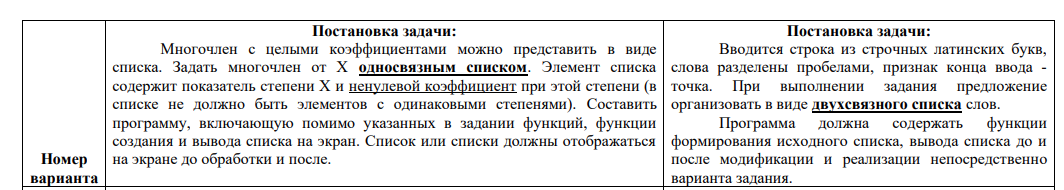
\includegraphics[width=1.1\linewidth]{images/task1}
	
	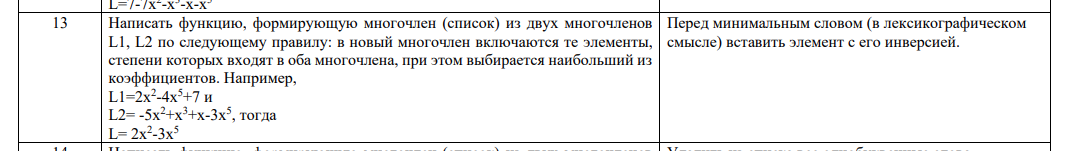
\includegraphics[width=1.1\linewidth]{images/task}

	
	\newpage
	
	\section{10.1}
	
	\begin{lstlisting}[language=C]
		#include <stdio.h> // Input/output library.
		#include <stdlib.h> // Memory allocation.
		#include <assert.h> // Assertion library.
		#include <string.h> // String functions library.
		
		struct M {
			long a;
			unsigned n;
		};
		typedef struct M M;
		
		struct PListItem {
			struct M* valueP;
			struct PListItem* nextP;
		};
		typedef struct PListItem PListItem;
		
		struct PList {
			PListItem* headP;
		};
		typedef struct PList PList;
		
		long parseStringToLongInt(char* s) {
			long out = 0;
			int placeholder10 = 1;
			int sLength = strlen(s);
			int k = 1;
			
			if (s[0] == '-') {
				k = -1;
			}
			
			for (int i = sLength - 1; i >= 0; i--) {
				if (s[i] == ' ' || s[i] < '0' || s[i] > '9') {
					continue;
				}
				
				out += k * placeholder10 * (s[i] - '0');
				placeholder10 *= 10;
			}
			
			return out;
		}
		
		void printPList(PList* pListP) {
			PListItem* cur = pListP->headP;
			
			if (cur == NULL) {
				printf("unfortunately this polynomial list is incorrect or empty =(\n");
			}
			
			char tmp = '+';
			
			while (cur != NULL) {
				if (cur->valueP->a < 0) {
					tmp = 0;
				} else {
					tmp = '+';
				}
				
				printf("%c%ldx^%u", tmp, cur->valueP->a, cur->valueP->n);
				
				cur = cur->nextP;
			}
			
			printf("\n");
		}
		
		PListItem* findWithSameN(PList* pList, int n) {
			PListItem* cur = pList->headP;
			
			while (cur != NULL) {
				if (cur->valueP->n == n) {
					return cur;
				}
				
				cur = cur->nextP;
			}
			
			return NULL;
		}
		
		PListItem* clearPListItem(PListItem* pListItem) {
			PListItem* nextP = pListItem->nextP;
			
			free(pListItem->valueP);
			free(pListItem);
			
			return nextP;
		}
		
		PList* clearPList(PList* pList) {
			PListItem* cur = pList->headP;
			
			while (cur != NULL) {
				cur = clearPListItem(cur);
			}
			
			free(pList);
			pList = NULL;
			
			return pList;
		}
		
		void clearMonomWithA0(PList* pList) {
			PListItem* cur = pList->headP->nextP;
			PListItem* prev = pList->headP;
			
			while (cur != NULL) {
				if (cur->valueP->a == 0) {
					prev->nextP = cur->nextP;
					clearPListItem(cur);
				} else {
					prev = prev->nextP;
				}
				
				cur = prev->nextP;
			}
			
			if (pList->headP->valueP->a == 0) {
				cur = pList->headP;
				pList->headP = pList->headP->nextP;
				clearPListItem(cur);
			}
		}
		
		PList* parsePStringToPList(char* pStringP) {
			PList* out = (PList*)malloc(sizeof(PList));
			out->headP = (PListItem*)malloc(sizeof(PListItem));
			out->headP = NULL;
			
			if (pStringP[0] == 0) {
				return out;
			}
			
			PListItem* sameNCandidate = NULL;
			PListItem* prev = NULL;
			PListItem* cur = (PListItem*)malloc(sizeof(PListItem));
			cur->valueP = (M*)malloc(sizeof(M));
			cur->nextP = NULL;
			
			char placeholderP[100] = "";
			
			for (int i = 0; pStringP[i] != 0; i++) {
				if (pStringP[i] == ' ') {
					continue;
				}
				
				if ((pStringP[i] == '+' || pStringP[i] == '-')) {
					if (placeholderP[0] != 0) {
						cur->valueP->n = parseStringToLongInt(placeholderP);
						
						PListItem* sameNCandidate = findWithSameN(out, cur->valueP->n);
						
						if (sameNCandidate == NULL) {
							if (out->headP == NULL) {
								out->headP = cur;
							} else {
								prev->nextP = cur;
							}
							
							prev = cur;
						} else {
							sameNCandidate->valueP->a += cur->valueP->a;
							clearPListItem(cur);
						}
						
						cur = (PListItem*)malloc(sizeof(PListItem));
						cur->valueP = (M*)malloc(sizeof(M));
						cur->nextP = NULL;
					}
					
					placeholderP[0] = pStringP[i];
					placeholderP[1] = 0;
				}
				
				if (pStringP[i] == 'x') {
					cur->valueP->a = parseStringToLongInt(placeholderP);
					assert(cur->valueP->a != 0);
					
					placeholderP[0] = 0;
				}
				
				if (pStringP[i] <= '9' && pStringP[i] >= '0') {
					placeholderP[strlen(placeholderP) + 1] = 0;
					placeholderP[strlen(placeholderP)] = pStringP[i];
				} else if (
				pStringP[i] != 'x'
				&& pStringP[i] != '+'
				&& pStringP[i] != '-'
				&& pStringP[i] != '^'
				) {
					out->headP = NULL;
					return out;
				}
			}
			
			cur->valueP->n = parseStringToLongInt(placeholderP);
			
			sameNCandidate = findWithSameN(out, cur->valueP->n);
			
			if (sameNCandidate == NULL) {
				if (out->headP == NULL) {
					out->headP = cur;
				} else {
					prev->nextP = cur;
				}
			} else {
				sameNCandidate->valueP->a += cur->valueP->a;
				clearPListItem(cur);
			}
			
			clearMonomWithA0(out);
			
			return out;
		}
		
		void copyPListItem(PListItem* new, PListItem* cur) {
			new->nextP = NULL;
			new->valueP->a = cur->valueP->a;
			new->valueP->n = cur->valueP->n;
		}
		
		PList* mixTwoPLists(PList* pListP1, PList* pListP2) {
			PList* out = (PList*)malloc(sizeof(PList));
			
			PListItem* cur1 = pListP1->headP;
			PListItem* cur2 = pListP2->headP;
			
			PListItem* prevGood = NULL;
			
			out->headP = NULL;
			
			while (cur1 != NULL) {
				cur2 = pListP2->headP;
				
				while (cur2 != NULL && cur2->valueP->n != cur1->valueP->n) {
					cur2 = cur2->nextP;
				}
				
				if (cur2 != NULL) {
					PListItem* curGood = (PListItem*)malloc(sizeof(PListItem));
					curGood->valueP = (M*)malloc(sizeof(M));
					
					if (cur2->valueP->a >= cur1->valueP->a) {
						copyPListItem(curGood, cur2);
					} else {
						copyPListItem(curGood, cur1);
					}
					
					if (out->headP == NULL) {
						out->headP = curGood;
					} else {
						prevGood->nextP = curGood;
					}
					
					prevGood = curGood;
				}
				
				cur1 = cur1->nextP;
			}
			
			return out;
		};
		
		void readPStringFromUser(int pi, char* pStringP) {
			printf("Enter P%d: ", pi);
			
			fflush(stdin);
			fgets(pStringP, 100, stdin);
			pStringP[strcspn(pStringP, "\n")] = 0;
		}
		
		int main() {
			char* pStringP1 = (char*)malloc(100 * sizeof(char));
			char* pStringP2 = (char*)malloc(100 * sizeof(char));
			
			printf("Lab 10. Keyer, BAM231.\n");
			
			readPStringFromUser(1, pStringP1);
			readPStringFromUser(2, pStringP2);
			
			PList* pListP1 = parsePStringToPList(pStringP1);
			PList* pListP2 = parsePStringToPList(pStringP2);
			
			printPList(pListP1);
			printPList(pListP2);
			
			PList* finalPList = mixTwoPLists(pListP1, pListP2);
			
			printf("Polynomials mixin: ");
			printPList(finalPList);
			
			
			clearPList(pListP1);
			clearPList(pListP2);
			clearPList(finalPList);
			
			finalPList->headP = NULL;
			
			free(pStringP1);
			free(pStringP2);
			
			return 0;
		}
	\end{lstlisting}
	
		\section{10.1}
	
	\begin{lstlisting}[language=C]
		#include <stdio.h> // Input/output library.
		#include <stdlib.h> // Memory allocation.
		#include <string.h> // String functions library.
		
		struct WordListItem {
			char* valueP;
			struct WordListItem* nextP;
			struct WordListItem* prevP;
		};
		typedef struct WordListItem WordListItem;
		
		struct WordList {
			WordListItem* headP;
			WordListItem* tailP;
		};
		typedef struct WordList WordList;
		
		// Function validating a string.
		int isValid(char* s) {
			for (int i = 0; s[i] != 0; i++) {
				if ((s[i] < 'a' || s[i] > 'z') && s[i] != ' ' && s[i] != '.') {
					printf("String contains incorrect symbol: %c\n", s[i]);
					return 0;
				}
			}
			
			return 1;
		}
		
		WordList* parseStringToWordList(char* s) {
			WordList* out = (WordList*)malloc(sizeof(WordList));
			
			WordListItem* cur = (WordListItem*)malloc(sizeof(WordListItem));
			out->headP = cur;
			WordListItem* prev = NULL;
			
			cur->valueP = (char*)malloc(sizeof(char) * 100);
			cur->valueP[0] = 0;
			cur->prevP = NULL;
			
			for (int i = 0; s[i] != 0; i++) {
				if (s[i] != ' ') {
					cur->valueP[strlen(cur->valueP) + 1] = 0;
					cur->valueP[strlen(cur->valueP)] = s[i];
				} else {
					prev = cur;
					
					cur->nextP = (WordListItem*)malloc(sizeof(WordListItem));
					cur = cur->nextP;
					
					cur->prevP = prev;
					cur->valueP = (char*)malloc(sizeof(char) * 100);
					cur->valueP[0] = 0;
				}
			}
			
			cur->prevP = prev;
			cur->nextP = NULL;
			
			out->tailP = cur;
			
			return out;
		};
		
		void printWordList(WordList* wordList) {
			if (wordList->headP == NULL) {
				printf("Incorrect word list was input");
				return;
			}
			
			WordListItem* cur = wordList->headP;
			
			printf("Next direction: ");
			
			printf("%s", cur->valueP);
			cur = cur->nextP;
			
			while (cur != NULL) {
				printf(" %s", cur->valueP);
				cur = cur->nextP;
			}
			
			printf(".\n");
			
			printf("Prev direction: ");
			
			cur = wordList->tailP;
			
			printf("%s", cur->valueP);
			cur = cur->prevP;
			
			while (cur != NULL) {
				printf(" %s", cur->valueP);
				cur = cur->prevP;
			}
			
			printf(".\n");
		};
		
		char* inverseWord(char* word) {
			char* out = (char*)malloc(100 * sizeof(char));
			
			int wordLength = strlen(word);
			
			out[wordLength] = 0;
			
			for (int i = 0; word[i] != 0; i++) {
				out[wordLength - i - 1] = word[i];
			}
			
			return out;
		}
		
		WordListItem* findMinimumWordItem(WordList* wordList) {
			WordListItem* out = wordList->headP;
			WordListItem* good = out;
			WordListItem* cur = good;
			
			while (cur != NULL) {
				if (strcmp(cur->valueP, good->valueP) <= 0) {
					good = cur;
				}
				cur = cur->nextP;
			}
			
			return good;
		}
		
		void solution(char* s) {
			WordList* wordList = parseStringToWordList(s);
			
			WordListItem* minimumWordItem = findMinimumWordItem(wordList);
			WordListItem* insertItem = (WordListItem*)malloc(sizeof(WordListItem));
			
			insertItem->valueP = inverseWord(minimumWordItem->valueP);
			
			insertItem->prevP = minimumWordItem->prevP;
			insertItem->nextP = minimumWordItem;
			
			if (minimumWordItem->prevP) {
				minimumWordItem->prevP->nextP = insertItem;
			} else {
				wordList->headP = insertItem;
			}
			
			minimumWordItem->prevP = insertItem;
			
			printf("Modifed string:\n");
			printWordList(wordList);
		}
		
		// Function reading a string from stdin.
		char* readingStringFromUser() {
			printf("Please, enter correct string: ");
			
			char* s = (char*)malloc(sizeof(char) * 100);
			
			fflush(stdin);
			fgets(s, 100, stdin);
			s[strcspn(s, "\n")] = 0;
			s[strcspn(s, ".")] = 0;
			
			return s;
		};
		
		int main() {
			char* s = readingStringFromUser();
			
			if (!isValid(s)) {
				return 1;
			}
			
			printf("Work with string: %s.\n", s);
			solution(s);
			
			free(s);
			return 0;
		};
	\end{lstlisting}
	
	\section{Тесты}
	
	\section{10.1}
	
	\subsection{Тест 1}

	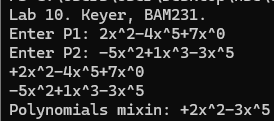
\includegraphics[width=\linewidth]{images/test1}
	
	С базовым тестом все нормик и работает! Проверим корнер кейсы.
	
		
	\subsection{Тест 2}
	
	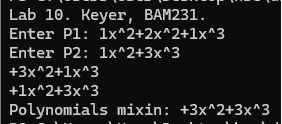
\includegraphics[width=\linewidth]{images/test2}
	
	Тут, как и ожидалось, слагаемые в P1 с одинаковыми степенями сложились.
	
	\subsection{Тест 3}
	
	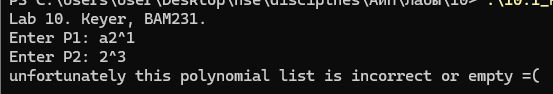
\includegraphics[width=\linewidth]{images/test3}
	
	Ругаемся, если введены неправильные символы или что-то противоречащее условиям задания.
	
	\section{10.2}

		\subsection{Тест 1}
	
	
	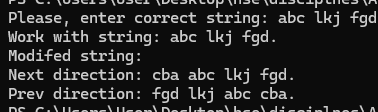
\includegraphics[width=\linewidth]{images/test4}
	
	С базовым тестом все нормик и работает! Проверим корнер кейсы.
	
	
	\subsection{Тест 2}
	
	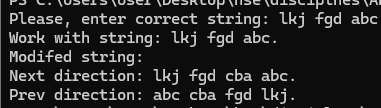
\includegraphics[width=\linewidth]{images/test5}
	
	Тут все, как и ожидалось.
	
	\subsection{Тест 3}
	
	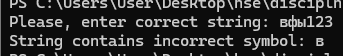
\includegraphics[width=\linewidth]{images/test6}
	
	Ругаемся, если введены неправильные символы или что-то противоречащее условиям задания.
	
\end{document}
